\begin{outline}
\1 Login Page
  
  \2 The login-page prompts a user to log-in with a student id and password.
  Currently the set of user ids and passwords are independent of those used by
  Pomona College. Note however the system does consider security, and stores
  only password digests encrypted via \texttt{bcrypt}.
  \2 Before Room Draw:
    \3 Upon successful log-in, a student is notified that they do not yet have
    an assigned room. They are also provided with simple navigational
    instructions.
  \2 After Room Draw:
    \3 If a student belongs to a draw group that has successfully drawn into a
    collection, the student is brought to a landing page informing the student
    of such. This provides information as for the students with whom they will
    be living, and the rooms that are collectively assigned to the said group of
    students. GUI access to other features of the site is disabled.
    \3 Otherwise, if a student does not yet belong to a draw group successfully
    assigned to a collection, the web-app behaves as Room Draw has not yet been
    drawn.
    
\begin{figure}[H] \centering
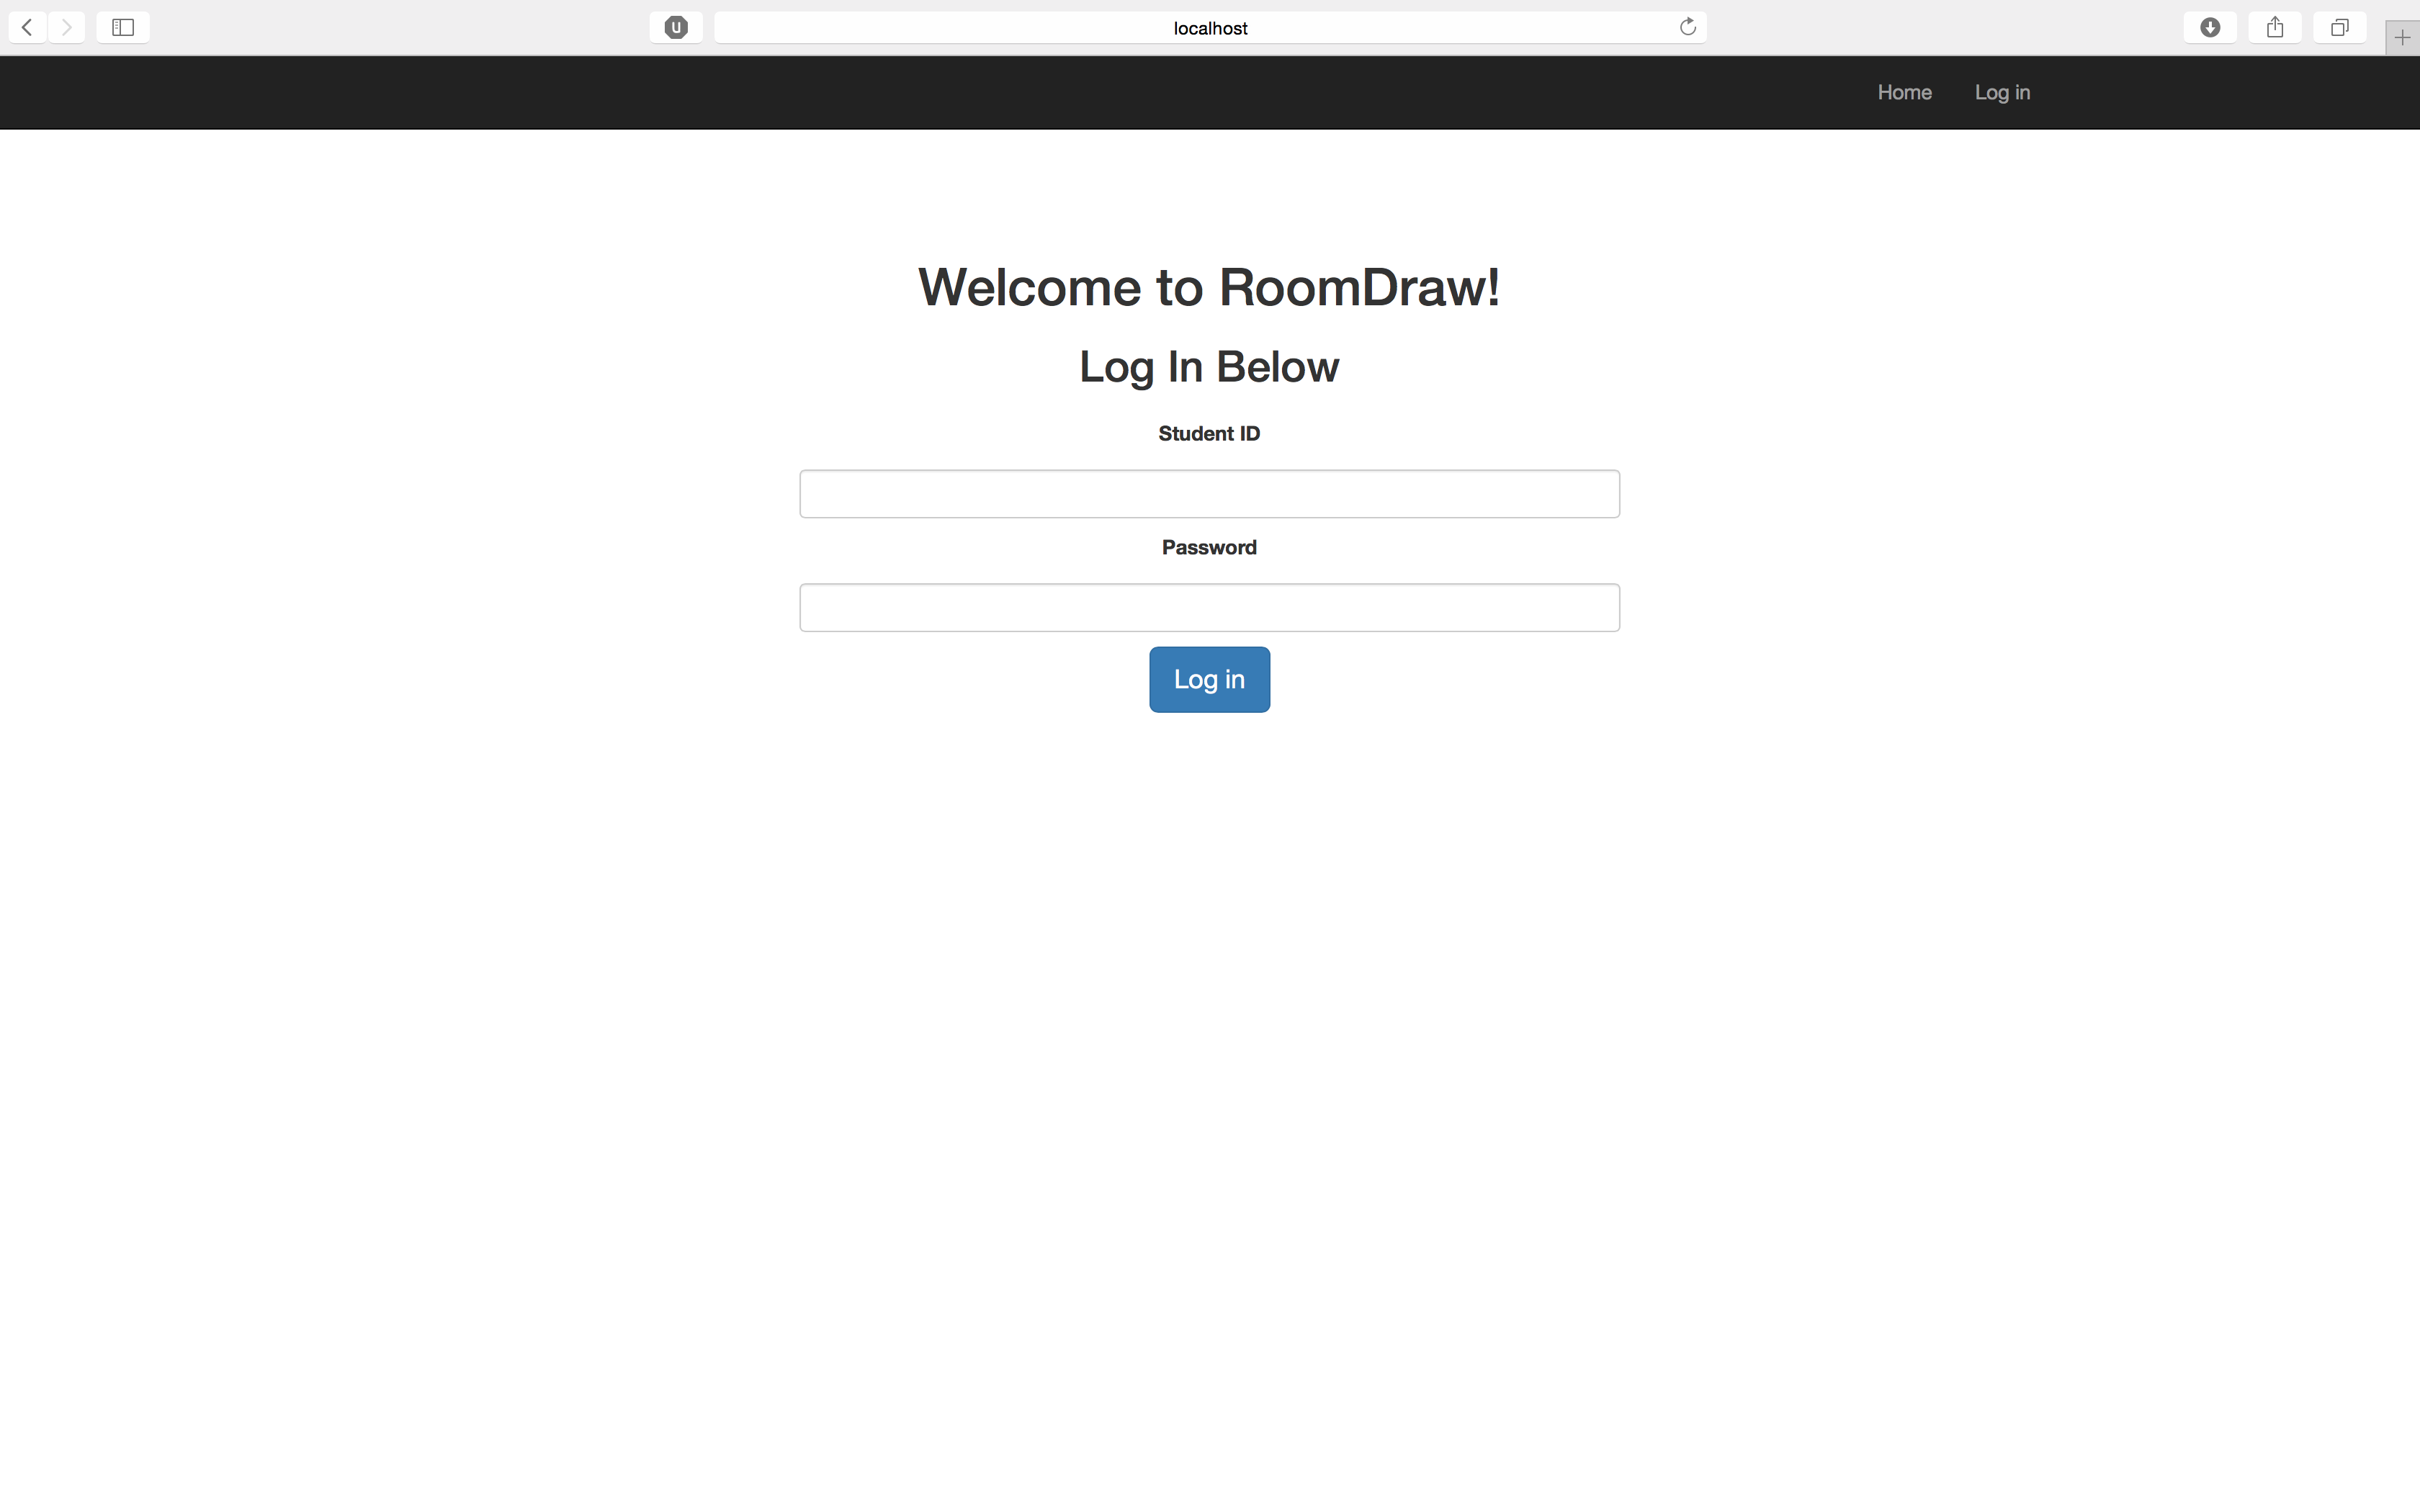
\includegraphics[scale=.225]{screens/login}
\caption{a login page}
\label{fig:screenlogin}
\end{figure}

\begin{figure}[H] \centering
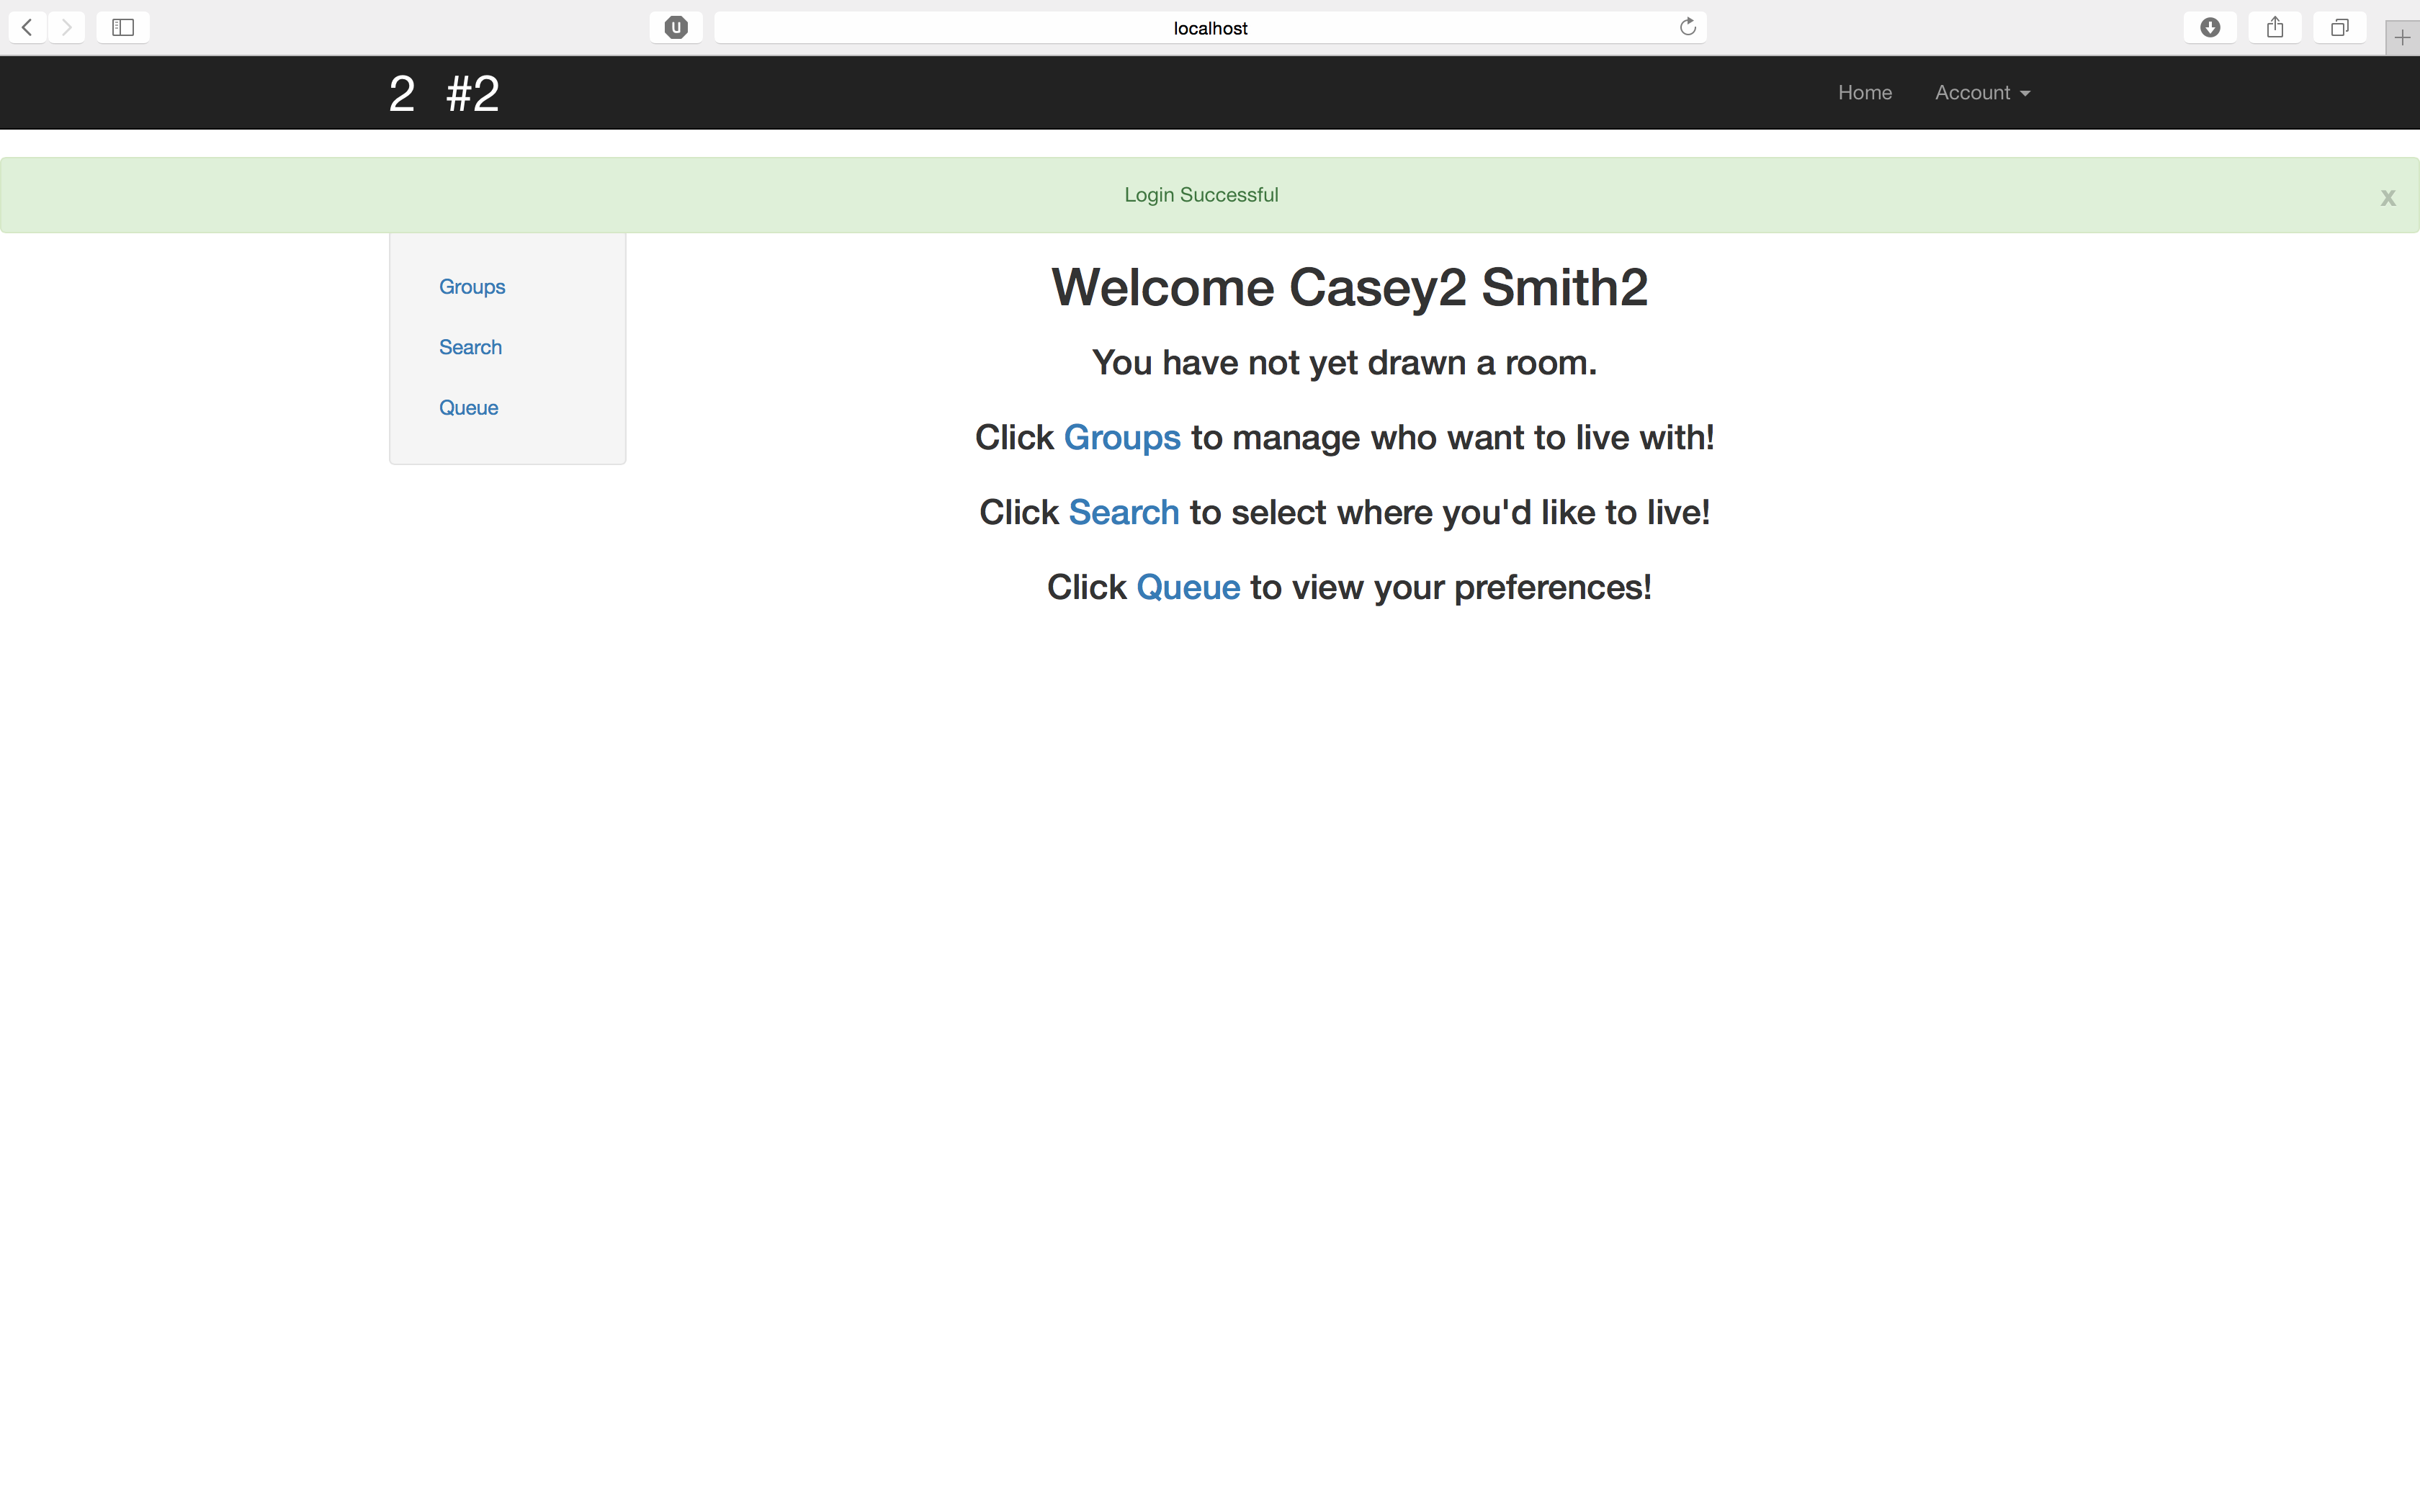
\includegraphics[scale=.225]{screens/landing_undrawn}
\caption{the landing page before room draw}
\label{fig:screenlandingundrawn}
\end{figure}

\begin{figure}[H] \centering
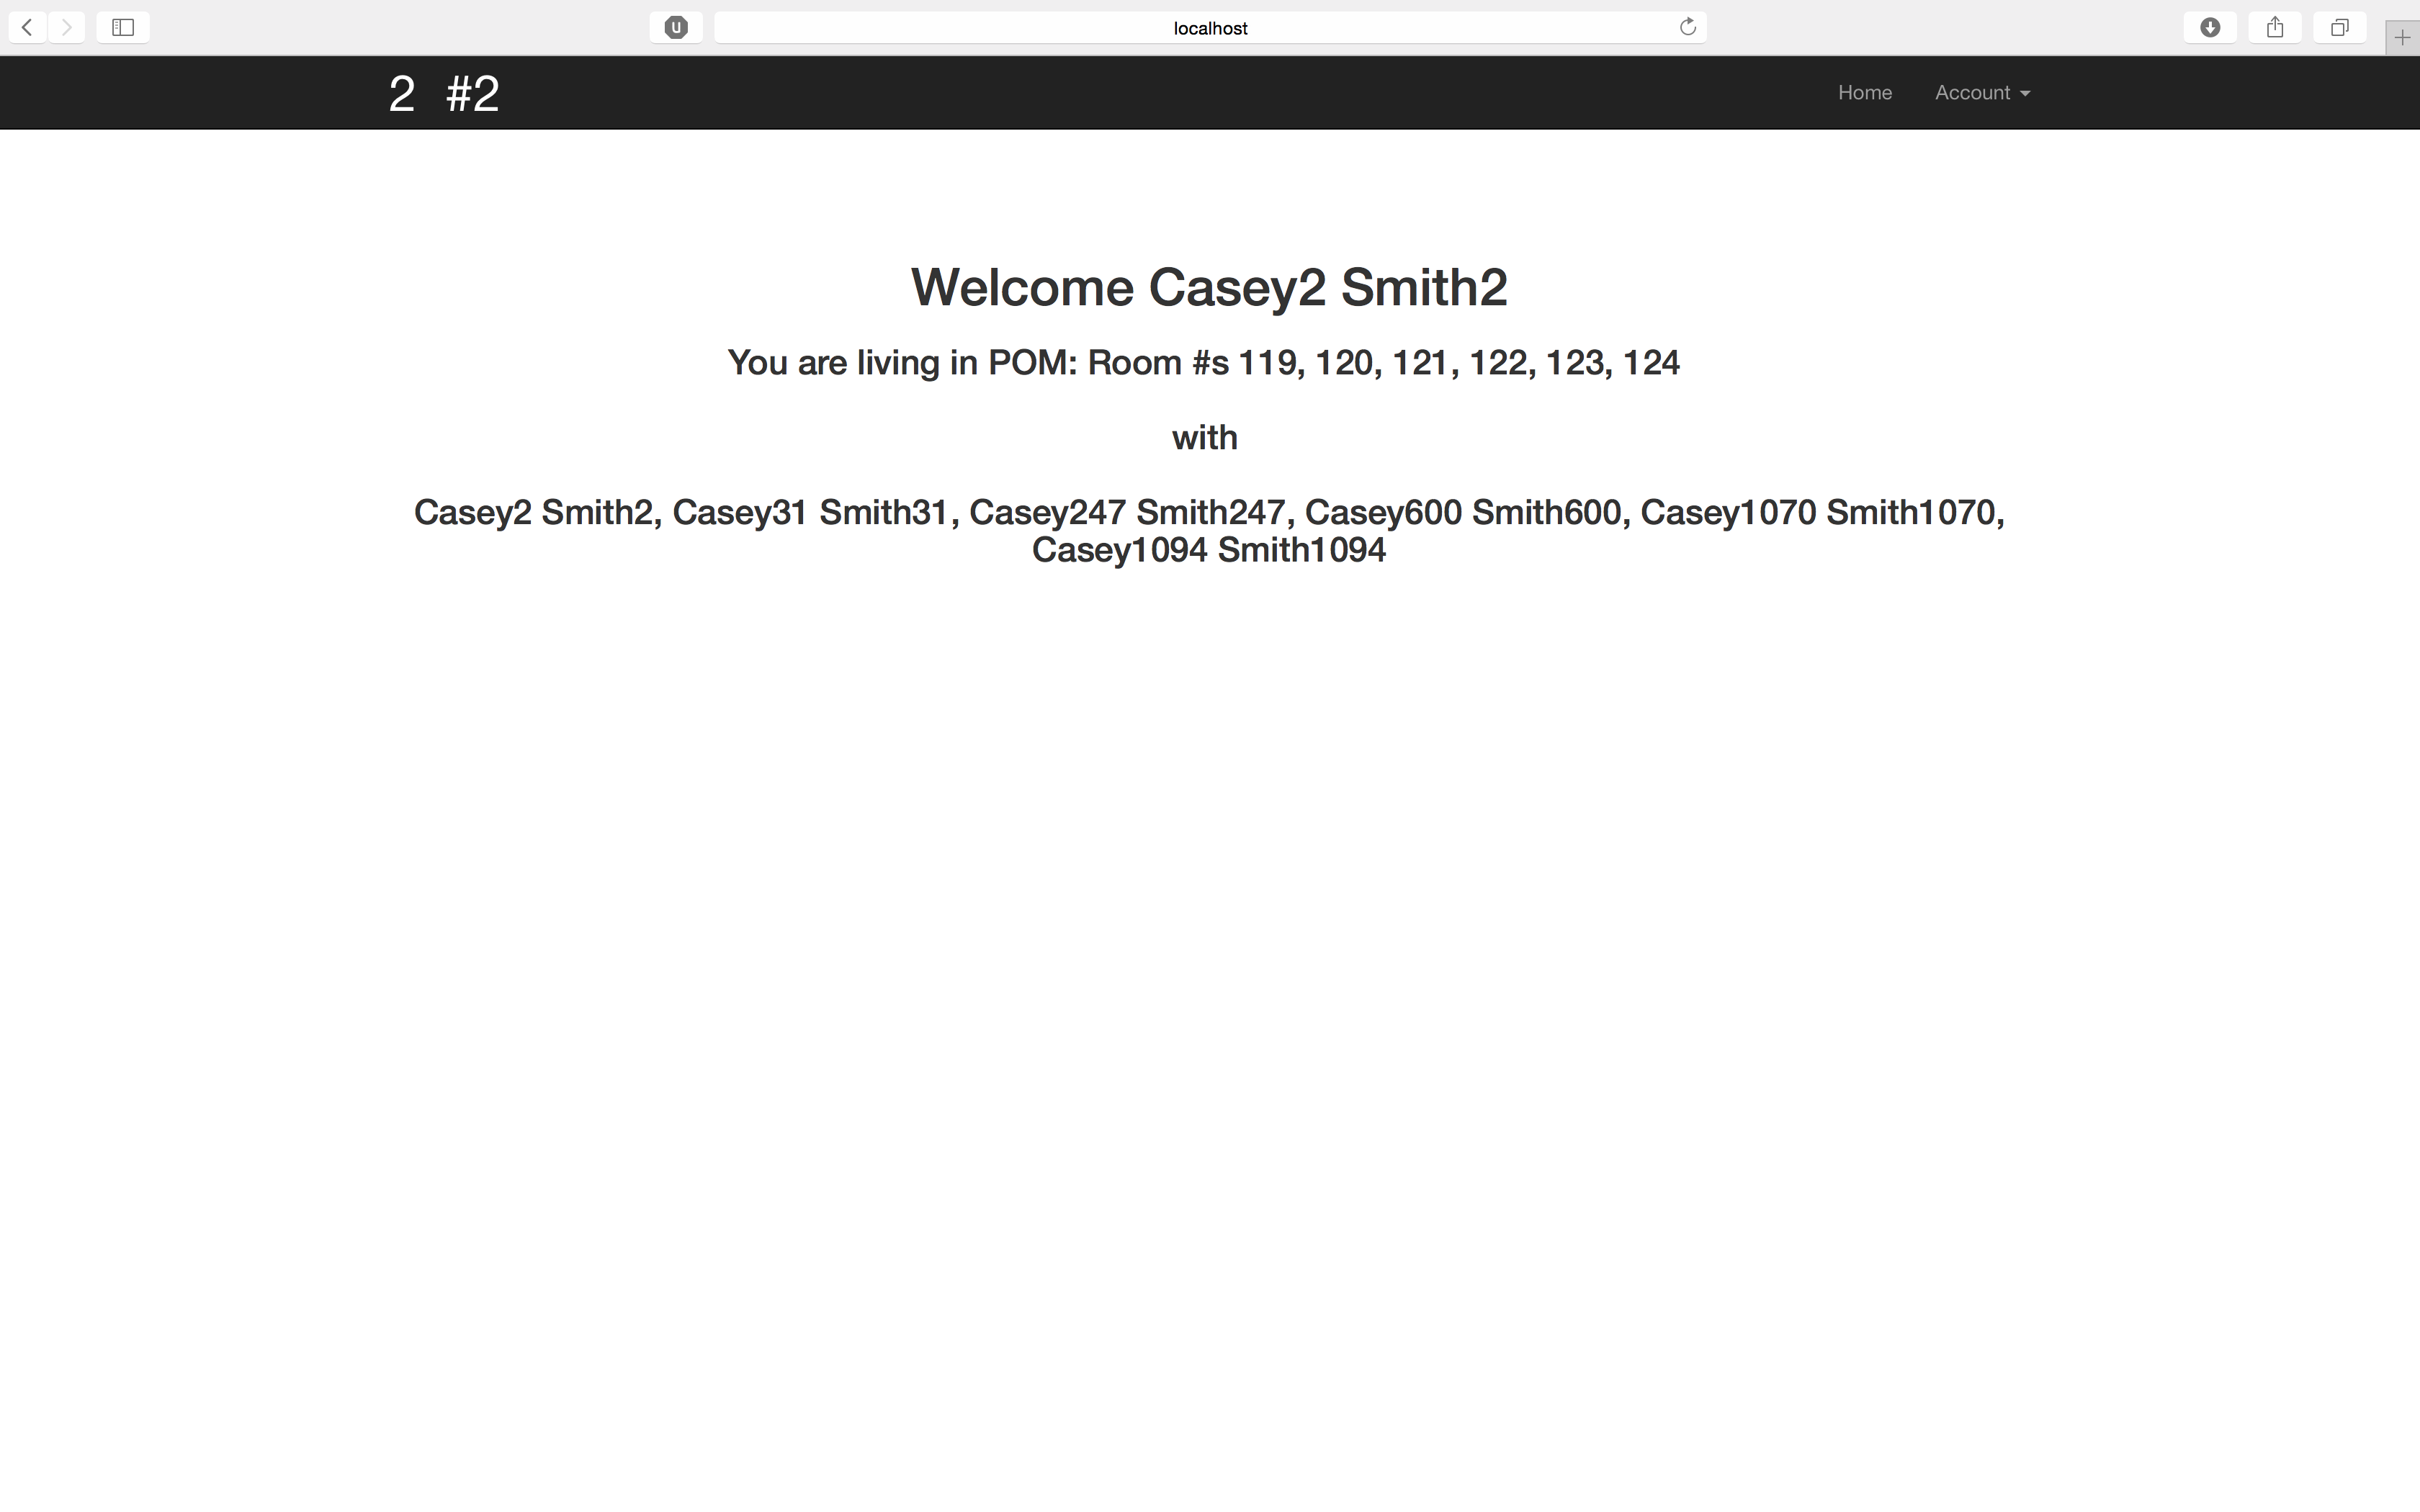
\includegraphics[scale=.225]{screens/landing_drawn}
\caption{the landing page after room draw}
\label{fig:screenlandingdrawn}
\end{figure}
    
\1 Group Management

  \2 By default, all students belong to a group containing only themselves.
  \2 All students may create additional draw groups (up to a max of 50). Doing
  so will create a new draw group, initialized containing the logged-in student.
  \2 Any student belonging to a draw group may add any other student to that
  group via student id. Draw groups are capped at size 6. Draw groups containing
  between 3 and 6 members are considered friendship groups, and have their draw
  numbers calculated accordingly.
  \2 Any student belonging to a group may delete it, which removes all data
  associated with that group.

\begin{figure}[H] \centering
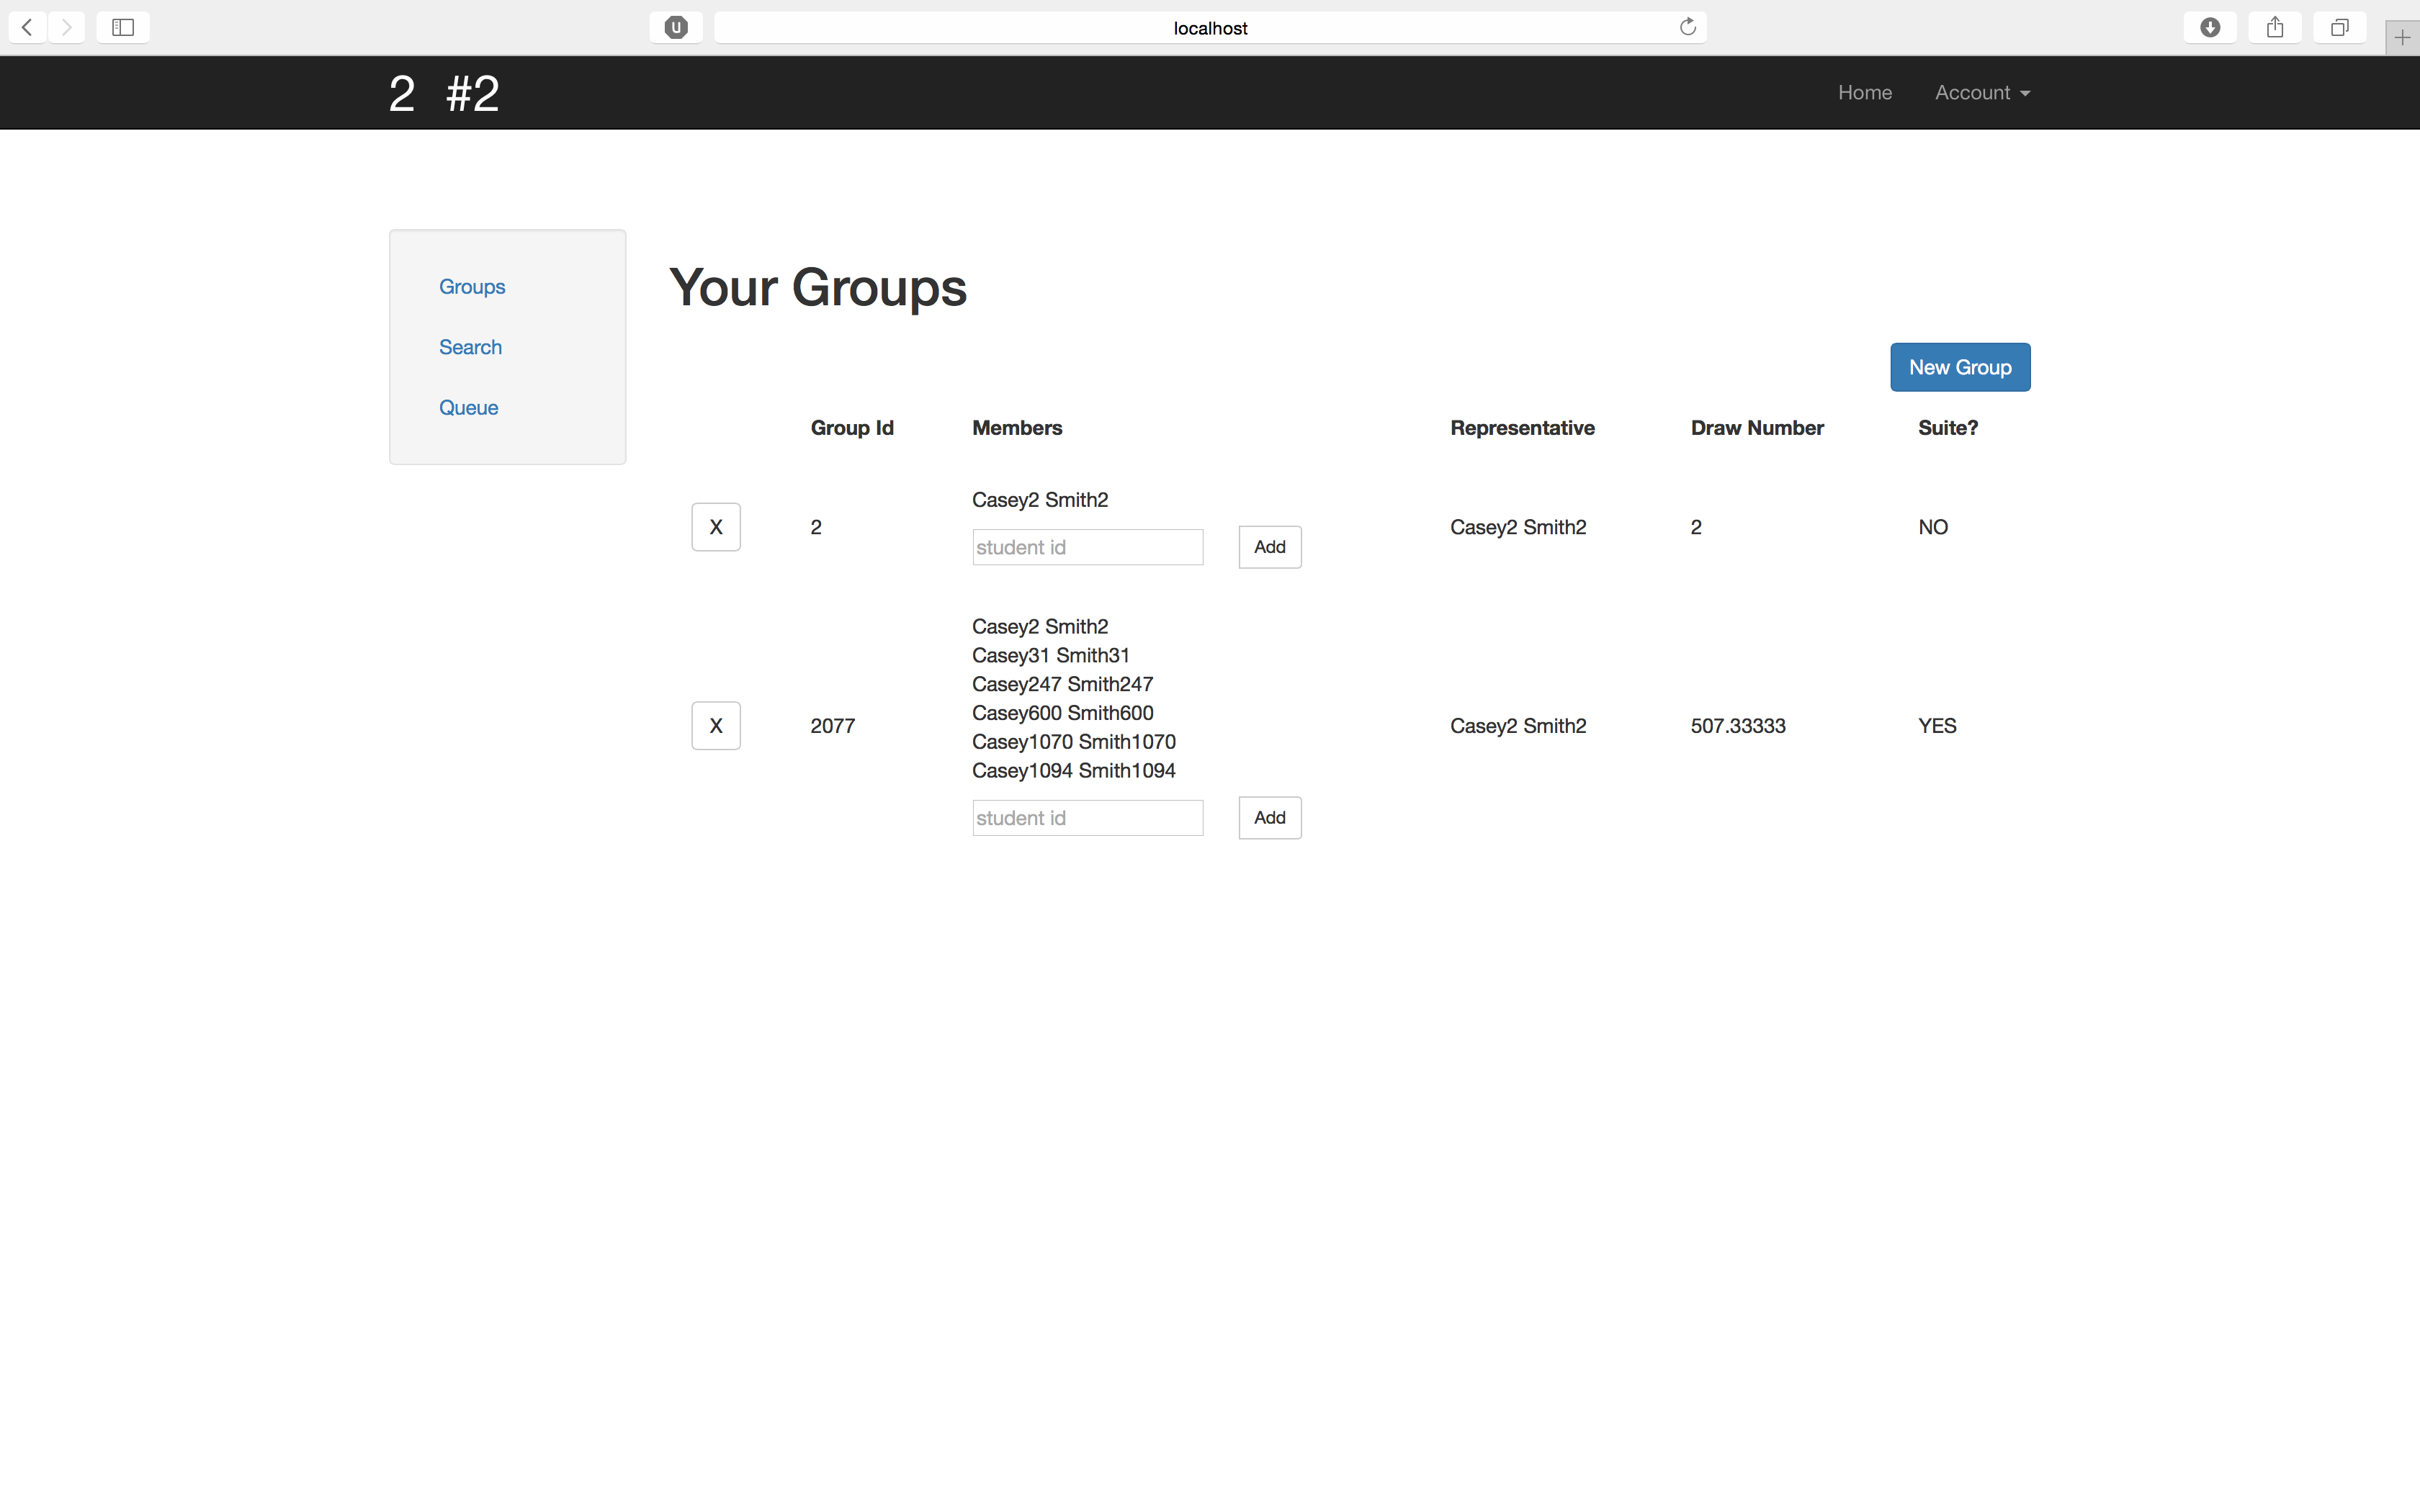
\includegraphics[scale=.225]{screens/group}
\caption{a page to manage one's groups}
\label{fig:screengroup}
\end{figure}
  
\1 Collection Search

  \2 The search page supports search by dorm name and by collection capacity.
  For each matching collection, the collection id, dorm name, room number(s),
  and room capacity(-ies) are listed. Group representatives may select a group
  they represent and add it to that group's preferences queue.

\begin{figure}[H] \centering
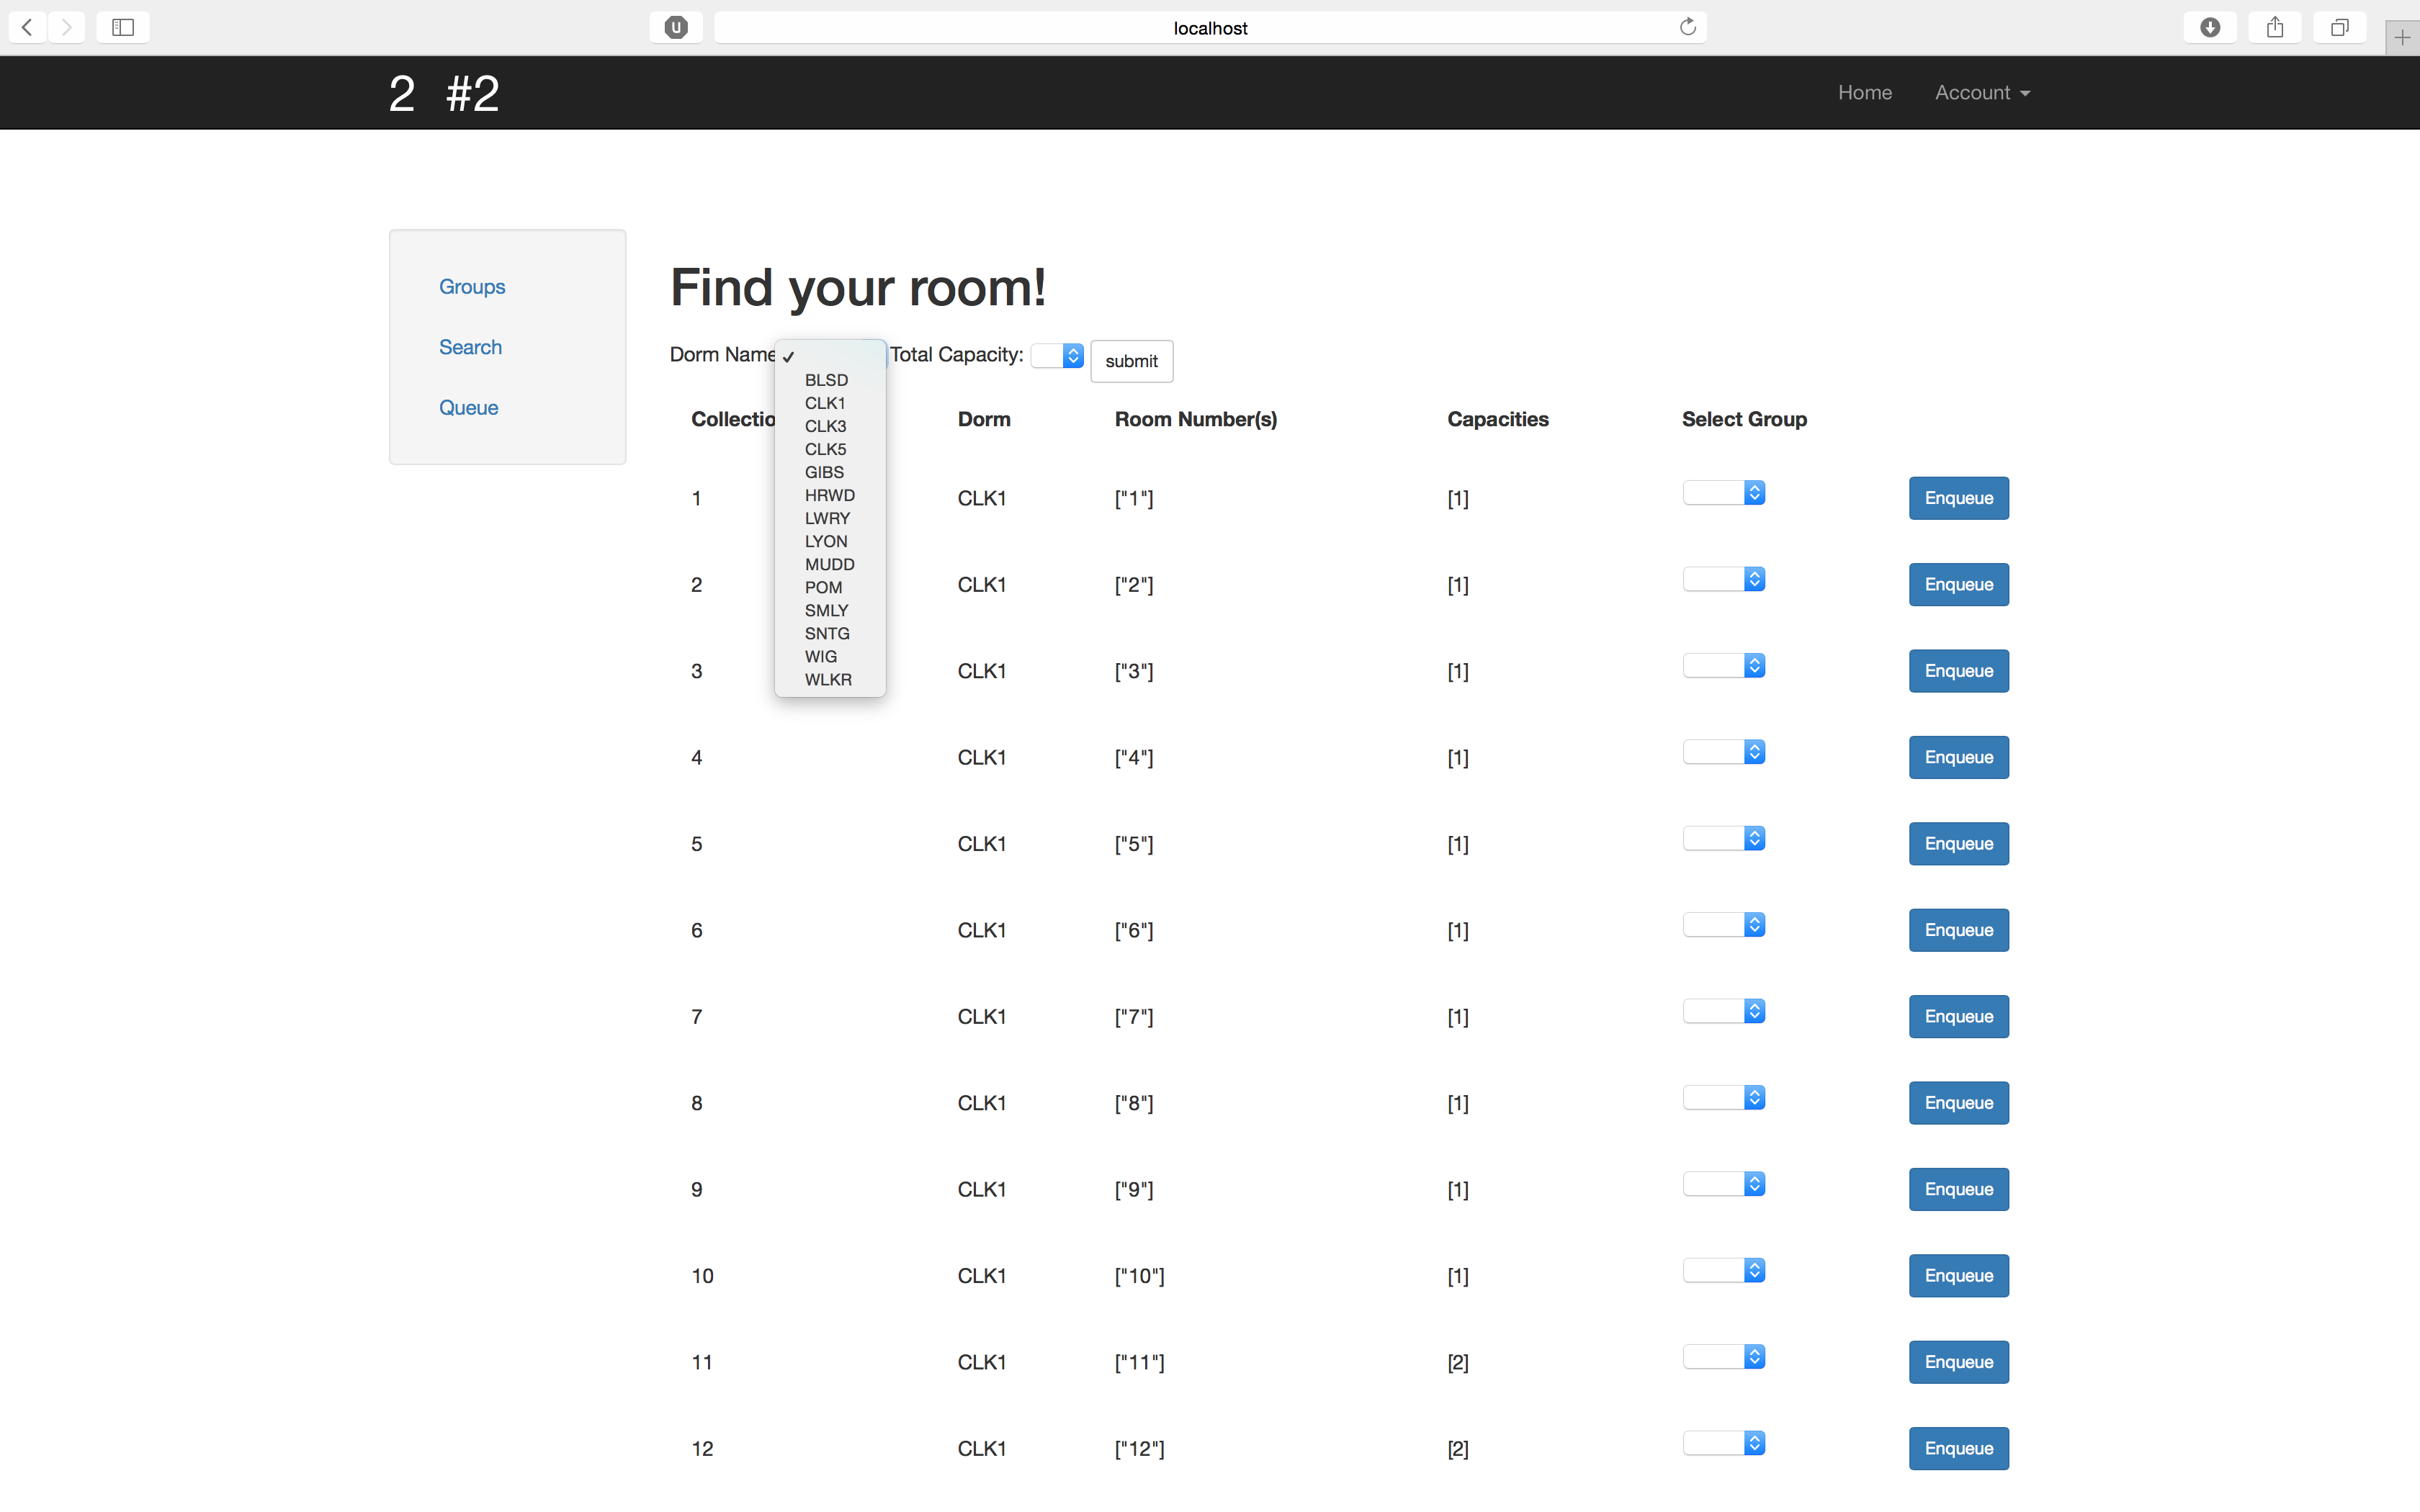
\includegraphics[scale=.225]{screens/search}
\caption{a page to filter through dorm listings and add them to one's queue}
\label{fig:screensearch}
\end{figure}

\1 Preference Queue

  \2 The Queue page lists out the various requests made by groups to which the
  logged-in student belongs. These requests are sorted first by the draw numbers
  of the groups, then by their addition time to the queue. We offer a small
  example to illustrate our intent: Consider that I add to my queue collection
  \(a\) for my solo group. I then add to my queue collection \(b\) for a
  friendship group I represent. I lastly add collection \(c\) for my solo group.
  The queue will display results in order \(b, a, c\), mirroring the order by
  which the requests would be evaluated at the moment of RoomDraw.
  \2 Requests in the queue may be deleted.
  
\begin{figure}[H] \centering
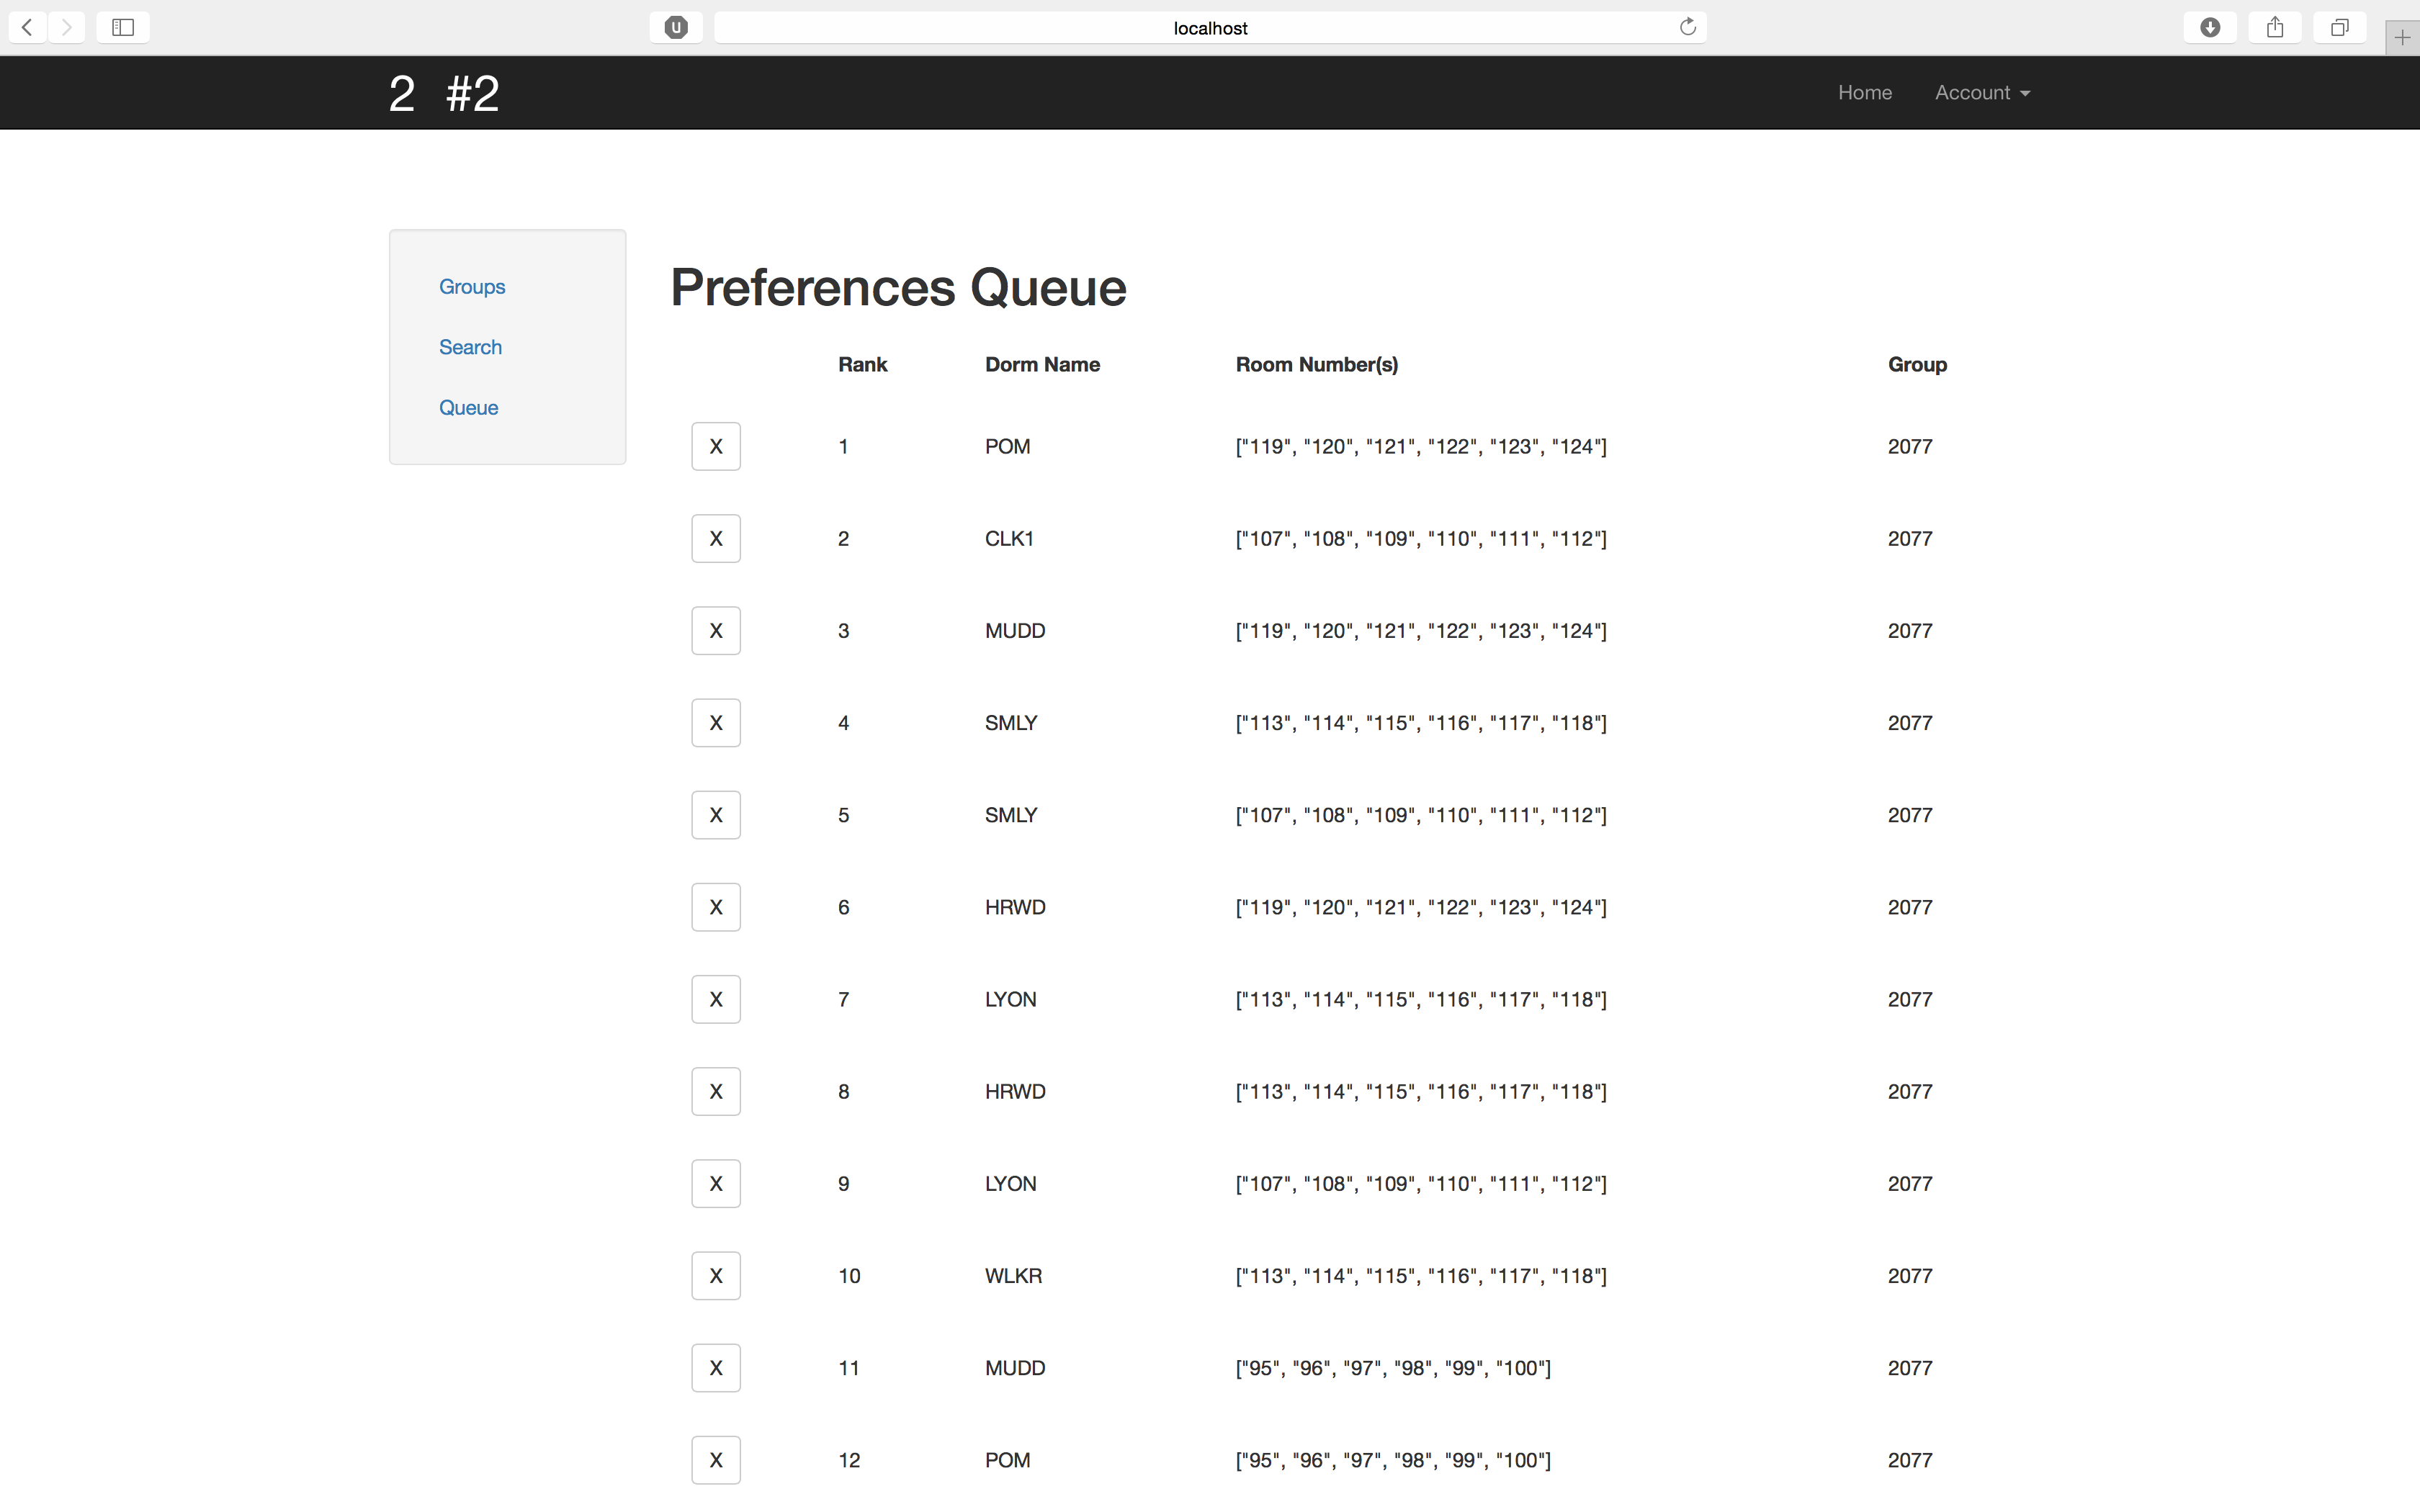
\includegraphics[scale=.225]{screens/queue}
\caption{a page to sort one's room collection preferences to automate the
    drawing process}
\label{fig:screenqueue}
\end{figure}
  
\end{outline}
